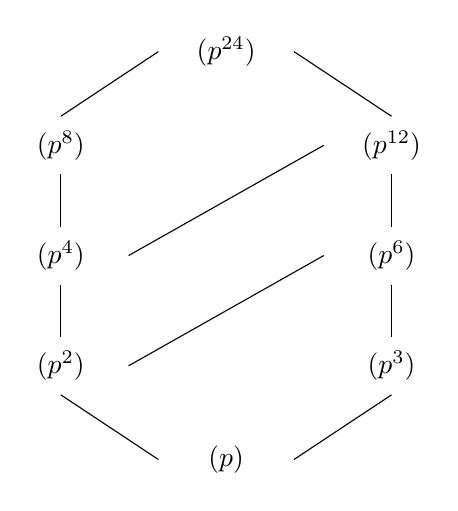
\begin{tikzpicture}[scale=0.7]

\coordinate (gf-p-24) at (0,3.7);
\coordinate (gf-p-8) at (-3,2);
\coordinate (gf-p-12) at (3,2);
\coordinate (gf-p-4) at (-3,0);
\coordinate (gf-p-6) at (3,0);
\coordinate (gf-p-2) at (-3,-2);
\coordinate (gf-p-3) at (3,-2);
\coordinate (gf-p) at (0,-3.7);

\node at (gf-p-24) {$\gf(p^{24})$};

\node at (gf-p-8) {$\gf(p^{8})$};
\node at (gf-p-12) {$\gf(p^{12})$};

\node at (gf-p-4) {$\gf(p^{4})$};
\node at (gf-p-6) {$\gf(p^{6})$};

\node at (gf-p-2) {$\gf(p^{2})$};
\node at (gf-p-3) {$\gf(p^{3})$};

\node at (gf-p) {$\gf(p)$};

\draw ([xshift=-35]gf-p-24) -- ([yshift=15]gf-p-8);
\draw ([xshift=35]gf-p-24) -- ([yshift=15]gf-p-12);

\draw ([yshift=-15]gf-p-8) -- ([yshift=15]gf-p-4);
\draw ([yshift=-15]gf-p-12) -- ([yshift=15]gf-p-6);
\draw ([xshift=-35]gf-p-12) -- ([xshift=35]gf-p-4);

\draw ([yshift=-15]gf-p-4) -- ([yshift=15]gf-p-2);
\draw ([yshift=-15]gf-p-6) -- ([yshift=15]gf-p-3);
\draw ([xshift=-35]gf-p-6) -- ([xshift=35]gf-p-2);

\draw ([yshift=-15]gf-p-2) -- ([xshift=-35]gf-p);
\draw ([yshift=-15]gf-p-3) -- ([xshift=35]gf-p);





\end{tikzpicture}


